% OpenAI Math Digest; follows the existing Schnell diagram style.
\documentclass[border=12pt]{standalone}
\def\pgfsysdriver{pgfsys-dvisvgm.def}
\usepackage[dvisvgm]{xcolor}
\usepackage{xeCJK}
\setCJKmainfont{HaranoAjiGothic-Regular.otf}[BoldFont=HaranoAjiGothic-Bold.otf]
\setCJKsansfont{HaranoAjiGothic-Regular.otf}[BoldFont=HaranoAjiGothic-Bold.otf]
\usepackage{amsmath,amssymb,tikz,lmodern}
\usetikzlibrary{arrows.meta,positioning,calc}
\renewcommand{\familydefault}{\sfdefault}
\definecolor{ink}{HTML}{25322F}
\definecolor{green}{HTML}{246657}
\definecolor{tint}{HTML}{EEF4F0}
\definecolor{soft}{HTML}{C6D2CC}
\definecolor{muted}{HTML}{52615B}
\definecolor{amber}{HTML}{866321}
\newif\ifJapanese
\newcommand{\Tx}[2]{\ifJapanese #1\else #2\fi}
\newcommand{\heading}[2]{{\color{green}\bfseries\Tx{#1}{#2}}\\[5pt]}
\newcommand{\refurl}[2]{\special{dvisvgm:raw <a xlink:href="#1" target="_blank" rel="noopener noreferrer">}{\color{green}\underline{\strut #2}}\special{dvisvgm:raw </a>}}
\newcommand{\R}[2]{\expandafter\refurl\expandafter{\csname source#1\endcsname}{#2}}
\tikzset{
 card/.style={draw=soft,fill=white,rounded corners=2pt,align=left,text=ink,font=\fontsize{10.5}{14}\selectfont,inner xsep=12pt,inner ysep=10pt,text width=14.4cm},
 result/.style={card,draw=green,fill=tint,line width=.9pt},
 reason/.style={align=left,text=muted,font=\fontsize{9}{12}\selectfont,inner sep=0pt,text width=12.65cm},
 edge/.style={-{Stealth[length=2.4mm]},draw=green,line width=1pt},
}
\newcommand{\flow}[3]{
 \coordinate (#2-from) at ($(#1.south)+(-6.9,0)$);
 \coordinate (#2-to) at ($(#2.north)+(-6.9,0)$);
 \draw[edge] (#2-from)--(#2-to);
 \node[reason,anchor=west] at ($(#2-from)!.5!(#2-to)+(.55,0)$) {#3};
}

\expandafter\def\csname sourceWV\endcsname{https://github.com/openai/math/blob/fd4aeeb2ee4fc729c18d98444fed42fd0529eeeb/preprints/Logarithmic-Kodaira-dimension-and-whole-fiber-variation-September-26-2026/paper.pdf}
\expandafter\def\csname sourceOI\endcsname{https://github.com/openai/math/blob/fd4aeeb2ee4fc729c18d98444fed42fd0529eeeb/preprints/Orbifold-and-logarithmic-Iitaka-subadditivity-September-26-2026/paper.pdf}
\expandafter\def\csname sourcePH\endcsname{https://github.com/openai/math/blob/fd4aeeb2ee4fc729c18d98444fed42fd0529eeeb/preprints/Projective-Hodge-lines-and-ordinary-Iitaka-subadditivity-September-27-2026/paper.pdf}
\expandafter\def\csname sourceRA\endcsname{https://github.com/openai/math/blob/fd4aeeb2ee4fc729c18d98444fed42fd0529eeeb/preprints/The-reverse-logarithmic-Kodaira-inequality-and-additivity-September-26-2026/paper.pdf}
\expandafter\def\csname sourceLA\endcsname{https://github.com/openai/math/blob/adc7f1241b42e322a6451854ab7e4b4c146bf78a/preprints/Log-abundance-in-characteristic-zero-September-24-2026/paper.pdf}
\expandafter\def\csname sourceFuj\endcsname{https://www.math.kyoto-u.ac.jp/~fujino/weak-posi11.pdf}
\expandafter\def\csname sourceDel\endcsname{https://www.numdam.org/item/PMIHES_1971__40__5_0.pdf}
\expandafter\def\csname sourceDHP\endcsname{https://arxiv.org/pdf/1012.0493v2}
\expandafter\def\csname sourcePT\endcsname{https://arxiv.org/pdf/1409.5504v1}
\expandafter\def\csname sourceBCHM\endcsname{https://arxiv.org/pdf/math/0610203v2}
\expandafter\def\csname sourceKP\endcsname{https://sites.math.washington.edu/~kovacs/2013/papers/Kovacs_Patakfalvi__Projectivity.pdf}
\expandafter\def\csname sourceHan\endcsname{https://doi.org/10.1007/BF01394338}
\expandafter\def\csname sourceSGA1\endcsname{https://arxiv.org/abs/math/0206203v2}
\expandafter\def\csname sourceLan\endcsname{https://arxiv.org/pdf/2005.09690v3}
\expandafter\def\csname sourceBDPP\endcsname{https://arxiv.org/pdf/math/0405285v1}
\expandafter\def\csname sourceTaj\endcsname{https://arxiv.org/pdf/2005.01025v4}
\Japanesefalse
\begin{document}
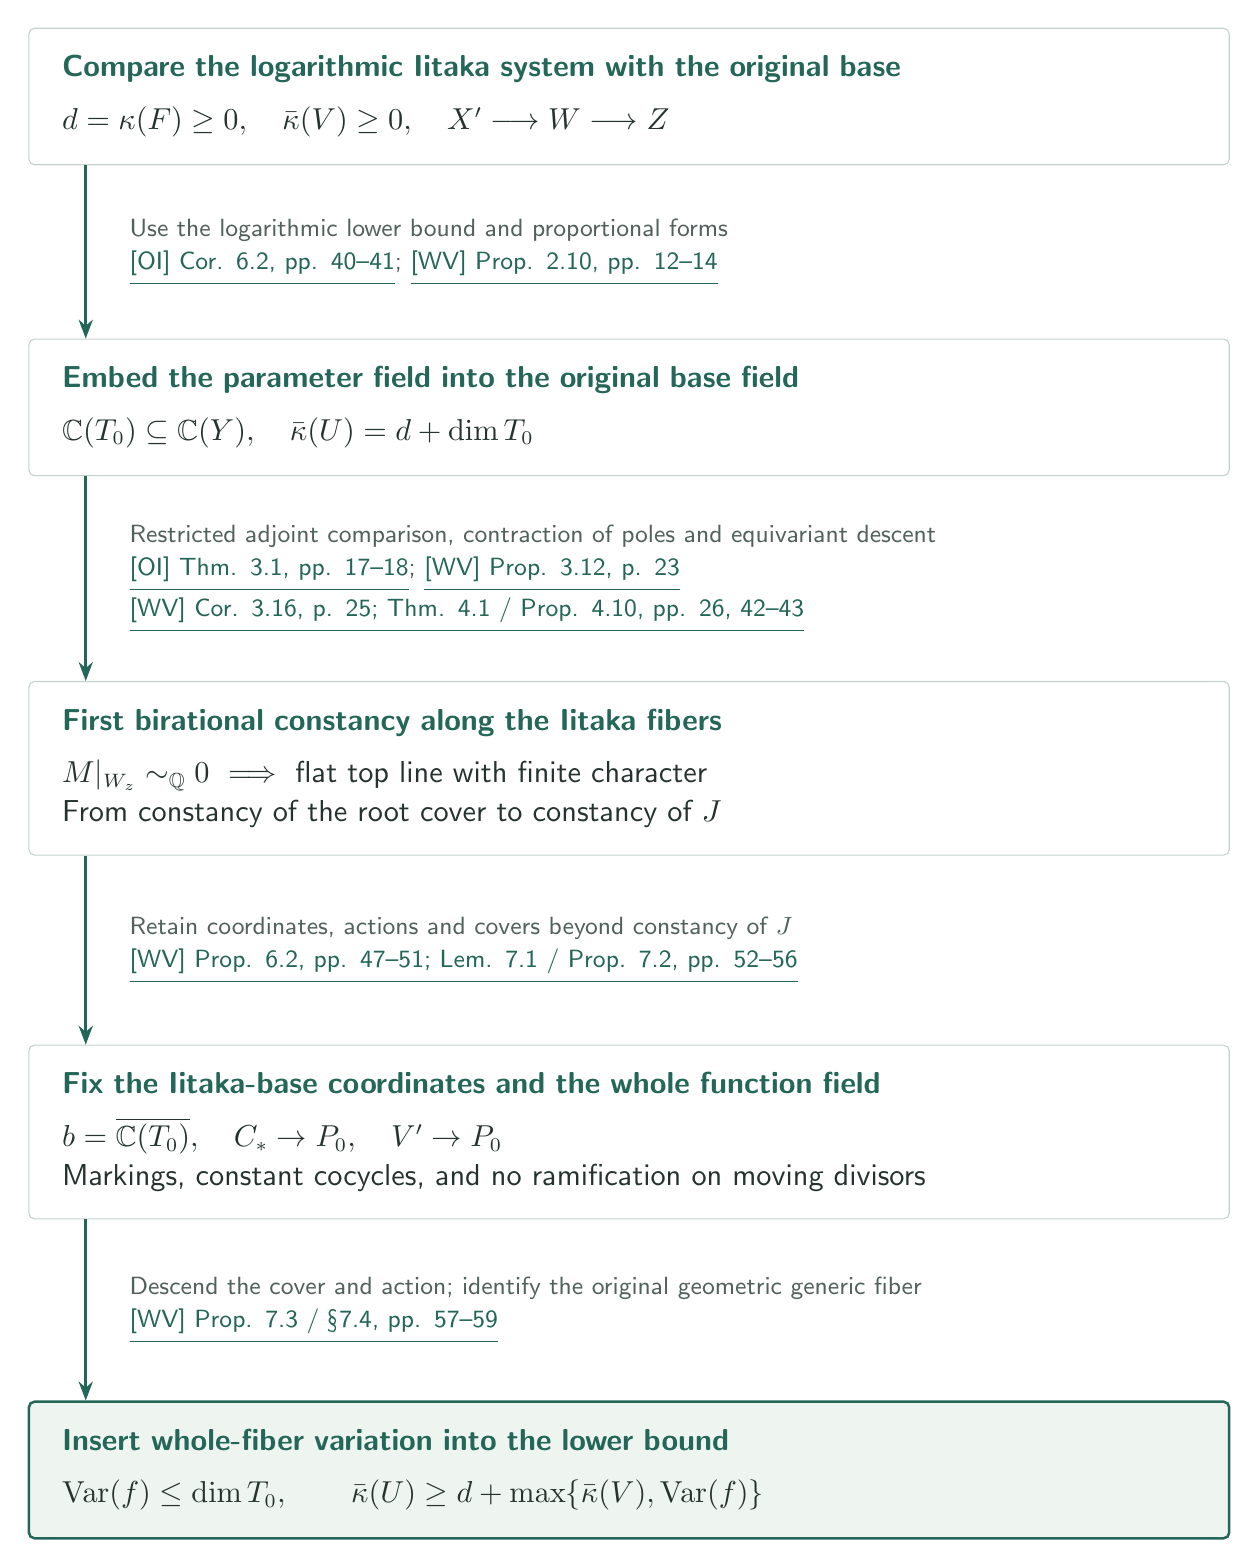
\begin{tikzpicture}
\node[card] (a) {\heading{対数的飯高系を元の底と比較する}{Compare the logarithmic Iitaka system with the original base}
 $d=\kappa(F)\ge0,\quad \bar\kappa(V)\ge0,\quad X'\longrightarrow W\longrightarrow Z$};
\node[card,below=2.2cm of a] (b) {\heading{parameter fieldを底の関数体に埋め込む}{Embed the parameter field into the original base field}
 $\mathbb C(T_0)\subseteq\mathbb C(Y),\quad\bar\kappa(U)=d+\dim T_0$};
\flow{a}{b}{\Tx{対数下界と形式の比例性から像の族を測る}{Use the logarithmic lower bound and proportional forms}\\
 \R{OI}{[OI] Cor. 6.2, pp. 40--41}; \R{WV}{[WV] Prop. 2.10, pp. 12--14}}
\node[card,below=2.6cm of b] (c) {\heading{飯高ファイバー方向で最初の双有理的constancy}{First birational constancy along the Iitaka fibers}
 $M|_{W_z}\sim_{\mathbb Q}0\ \Longrightarrow\ \Tx{\text{最高lineは平坦・有限指標}}{\text{flat top line with finite character}}$\\
 \Tx{root coverのconstancyから$J$のconstancyへ}{From constancy of the root cover to constancy of $J$}};
\flow{b}{c}{\Tx{制限上の随伴比較、極の収縮、群作用を保つ降下}{Restricted adjoint comparison, contraction of poles and equivariant descent}\\
 \R{OI}{[OI] Thm. 3.1, pp. 17--18}; \R{WV}{[WV] Prop. 3.12, p. 23}\\
 \R{WV}{[WV] Cor. 3.16, p. 25; Thm. 4.1 / Prop. 4.10, pp. 26, 42--43}}
\node[card,below=2.4cm of c] (d) {\heading{飯高底の座標と全関数体を固定する}{Fix the Iitaka-base coordinates and the whole function field}
 $b=\overline{\mathbb C(T_0)},\quad C_*\to P_0,\quad V'\to P_0$\\
 \Tx{marking、定数cocycle、動く因子上の非分岐性}{Markings, constant cocycles, and no ramification on moving divisors}};
\flow{c}{d}{\Tx{$J$のconstancyだけで止めず、座標・作用・被覆を保つ}{Retain coordinates, actions and covers beyond constancy of $J$}\\
 \R{WV}{[WV] Prop. 6.2, pp. 47--51; Lem. 7.1 / Prop. 7.2, pp. 52--56}}
\node[result,below=2.3cm of d] (e) {\heading{全ファイバーのvariationを下界へ入れる}{Insert whole-fiber variation into the lower bound}
 $\operatorname{Var}(f)\le\dim T_0,\qquad
 \bar\kappa(U)\ge d+\max\{\bar\kappa(V),\operatorname{Var}(f)\}$};
\flow{d}{e}{\Tx{被覆と群作用を降下し、元の幾何学的一般ファイバーと同定}{Descend the cover and action; identify the original geometric generic fiber}\\
 \R{WV}{[WV] Prop. 7.3 / \S7.4, pp. 57--59}}
\end{tikzpicture}


\end{document}
